\documentclass[11.5pt]{article}
\usepackage{stat110}

\title{Multivariate Distributions, Covariance \& Correlation}
\sectionnum{7}

\author{\shira, \tim, \creds}

%\SOLUTION

\begin{document}

\maketitle

\begin{notes}

\begin{comment}
\section*{Introduction}
Sometimes we have more than one random variable of interest, and we want to study probabilities associated with all of the random variables. Instead of studying the distributions of $X_1, X_2, X_3$ separately, we can study the distribution of the multivariate vector $\textbf{X} = (X_1, X_2, X_3)$. Joint PDFs and CDFs are analogous to multivariate versions of univariate PDFs and CDFs. Usually joint PDFs and PMFs carry more information than the marginal ones do, because they account for the interactions between the various random variables. If, however, the random variables are independent, then the joint PMF/PDF is just the product of the marginals and we get no extra information by studying them jointly rather than marginally.

\section*{Joint Distributions}
Joint Probability of events $A$ and $B$: $P(A,B) = P(A \cap B)$

\begin{table}[h]\begin{center}
	\begin{tabular}{ccccc} \toprule
		\textbf{Joint CDF} & ~ & \textbf{Joint PMF} & ~ & \textbf{Joint PDF} \\  \midrule
		$F_{X, Y}(x, y) = P(X \leq x,Y \leq y)$ & ~ & $P(X=x, Y=y)$ & ~ & $f_{X,Y}(x,y) = \frac{\delta}{\delta x} \frac{\delta}{\delta y}F_{X, Y}(x, y)$ \\ \bottomrule
	\end{tabular}\end{center}
\end{table}

Both the Joint PMF and Joint PDF must be non-negative and sum/integrate to 1. ($\sum_x \sum_y P(X=x, Y=y) = 1$) ($\int_x\int_y f_{X,Y}(x,y) = 1$). Like in the univariate cause, you sum/integrate the PMF/PDF to get the CDF.

\section*{Conditional Distributions}
By Bayes' Rule, $P(A|B) = \frac{P(B|A)P(A)}{P(B)}$ Similar conditions apply to conditional distributions of random variables.\\

For discrete random variables:
\[P(Y=y|X=x) = \frac{P(X=x, Y=y)}{P(X=x)} = \frac{P(X=x|Y=y)P(Y=y)}{P(X=x)}\]
For continuous random variables:
\[f_{Y|X}(y|x) = \frac{f_{X,Y}(x, y)}{f_X(x)} = \frac{f_{X|Y}(x|y)f_Y(y)}{f_X(x)}\]

\newpage

\section*{Marginal Distributions}
Law of Total Probability says for an event $A$ and partition $B_1, B_2, ... B_n$: $P(A) = \sum_i P(A\cap B_i)$, which implies that we can find the marginal probability by integrating out the $B$'s.  \\ \\
To find the distribution of one (or more) random variables from a joint distribution, sum or integrate over the irrelevant random variables. \\

Getting the Marginal PMF from the Joint PMF
$$P(X = x) = \sum_y P(X=x, Y=y)$$
Getting the Marginal PDF from the Joint PMF
$$f_X(x) = \int_y f_{X, Y}(x, y) \diff y$$



\section*{Independence of Random Variables}
Review: $A$ and $B$ are independent if and only if either $P(A\cap B) = P(A)P(B)$ or $P(A|B) = P(A)$. \\

Similar conditions apply to determine whether random variables are independent - two random variables are independent if their joint distribution function is simply the product of their marginal distributions, or that the a conditional distribution of is the same as its marginal distribution. \\

In words, random variables $X$ and $Y$ are independent for all $x, y$, if and only if one of the following hold:
\begin{itemize}
	\itemsep -1mm
	\item Joint PMF/PDF/CDFs are the product of the Marginal PMF
	\item Conditional distribution of $X$ given $Y$ is the same as the marginal distribution of $X$
\end{itemize}

\begin{table}[htb]
	\begin{tabular}{ccc}
		$X$ and $Y$ (discrete) are independent  & $\Longleftrightarrow$ & $P(X \leq x, Y \leq y) = P(X \leq x)P(Y \leq y),  \forall x, y$ \\ 
		$X$ and $Y$ (discrete) are independent  & $\Longleftrightarrow$ & $P(X=x, Y=y) = P(X=x)P(Y=y),  \forall x, y$ \\ 
		$X$ and $Y$ (discrete) are independent  & $\Longleftrightarrow$ & $P(X=x | Y=y) = P(X=x),  \forall x, y$ \\ 
		$X$ and $Y$  (continuous) are independent  & $\Longleftrightarrow$ & $P(X \leq x, Y \leq y) = P(X \leq x)P(Y \leq y),  \forall x, y$ \\ 
		$X$ and $Y$  (continuous) are independent  & $\Longleftrightarrow$ & $f_{X, Y}(x, y) = f_X(x)f_Y(y), \forall x, y$ \\ 
		$X$ and $Y$  (continuous) are independent  & $\Longleftrightarrow$ & $f_{X|Y}(X|Y) = f_X(X), \forall x, y$ 
	\end{tabular}
\end{table}

\section*{Multivariate LotUS}
In one dimension, we have: $E(g(X)) = \sum_xg(x)P(X=x)$, or $E(g(X)) = \int_{-\infty}^{\infty}g(x)f_X(x) \diff x$\\ \\ 
For discrete random variables:
$$E(g(X, Y)) = \sum_x\sum_yg(x, y)P(X=x, Y=y)$$
For continuous random variables:
$$E(g(X, Y)) = \int_{-\infty}^{\infty}\int_{-\infty}^{\infty}g(x, y)f_{X,Y}(x, y) \diff x \diff y $$



% \section*{Maximum Likelihood Estimator}
% If you observe data from a distribution where you don't know the parameter, one method of estimating that parameter is using the Maximum Likelihood Estimator (MLE). The MLE of a parameter of a distribution is the value that makes the observed data under that distribution as likely as possible. This is achieved by maximizing the density evaluated at the observed data over the parameter space.
\end{comment}

\section*{Multinomial (Multivariate Discrete)}

	Review - Binomial is a simple case of multinomial.
	
	Let us say that the vector $\vec{\textbf{X}} = (X_1, X_2, X_3, \dots, X_k) \sim \textnormal{Mult}_k(n, \vec{p})$  where $\vec{p} = (p_1, p_2, \dots, p_k)$.
\begin{description}
	\item[Story] - We have $n$ items, and then can fall into any one of the $k$ buckets independently with the probabilities $\vec{p} = (p_1, p_2, \dots, p_k)$.
	\item[Example] - Let us assume that every year, 100 students in the Harry Potter Universe are randomly and independently sorted into one of four houses with equal probability. The number of people in each of the houses is distributed Mult$_4$(100, $\vec{p}$), where $\vec{p} = (.25, .25, .25, .25)$.
		Note that $X_1 + X_2 + \dots + X_4 = 100$, and they are dependent.
	\item[Multinomial Coefficient] The number of permutations of $n$ objects where you have $n_1, n_2, n_3 \dots, n_k$ of each of the different variants is the \textbf{multinomial coefficient}.
		\[{n \choose n_1n_2\dots n_k} = \frac{n!}{n_1!n_2!\dots n_k!}\]
	\item[Joint PMF] - For $n = n_1 + n_2 + \dots + n_k$
		\[P(X_1 = n_1, X_2 = n_2, \dots, X_k = x_k) = {n \choose n_1n_2\dots n_k}p_1^{n_1}p_2^{n_2}\dots p_k^{n_k}\]
	\item[Lumping] - If you lump together multiple categories in a multinomial, then it is still multinomial. A multinomial with two dimensions (success, failure) is a binomial distribution.
	\item[Marginal PMF and Lumping]
		\[X_i \sim \Bin(n, p_i)\]
		\[X_i + X_j \sim \Bin(n, p_i + p_j)\]
		\[X_1, X_2, X_3 \sim \Mult_3(n, (p_1, p_2, p_3)) \Longrightarrow X_1, X_2 + X_3 \sim \Mult_2(n, (p_1, p_2 + p_3))\]
		\[X_1, X_2, \dots, X_{k-1} | X_k = n_k \sim \Mult_{k-1}\left(n - n_k, \left(\frac{p_1}{1 - p_k}, \frac{p_2}{1 - p_k}, \dots, \frac{p_{k-1}}{1 - p_k}\right)\right)\]
\end{description}

\section*{Multivariate Uniform (Multivariate Continuous)}
If $\mathbf{X} = (X_1, X_2, \ldots X_n)$ where $X_i \sim \Unif(a_i, b_i)$, then $X$ is distributed multivariate uniform and can be thought of pictorally as a box in $n$ dimensions, where any point within the box is equally likely to be selected. \\
The PDF of any point inside the box (the support of $\mathbf{X}$) is equal to 1 over the volume of the box, so for all $\mathbf{x} \in \mathbb{R}^n$ in the box, we have:  

$$ f_{\mathbf{X}}(x) = \frac{1}{(b_1 - a_1) (b_2 - a_2) \ldots (b_n - a_n)}$$

An analogous result is true for the discrete case. The PMF at each point is simply 1 divided by the total number of points. 

\section*{Multivariate Normal (MVN)}
A vector $\vec{X} = (X_1, X_2, X_3, \dots, X_k)$ is declared Multivariate Normal if any linear combination is normally distributed (e.g. $t_1X_1 + t_2X_2 + \dots + t_kX_k$ is Normal for any constants $t_1, t_2, \dots, t_k$). The parameters of the Multivariate normal are the mean vector $\vec{\mu} = (\mu_1, \mu_2, \dots, \mu_k)$ and the covariance matrix $\Sigma$ where the $(i, j)^{\textnormal{th}}$ entry is $\cov(X_i, X_j)$. For any MVN distribution: 1) Any sub-vector is also MVN. 2) If any two elements of a multivariate normal distribution are uncorrelated, then they are independent. Note that this does not apply to most random variables. 

\section*{Covariance and Correlation}
\begin{figure}[h]\centering
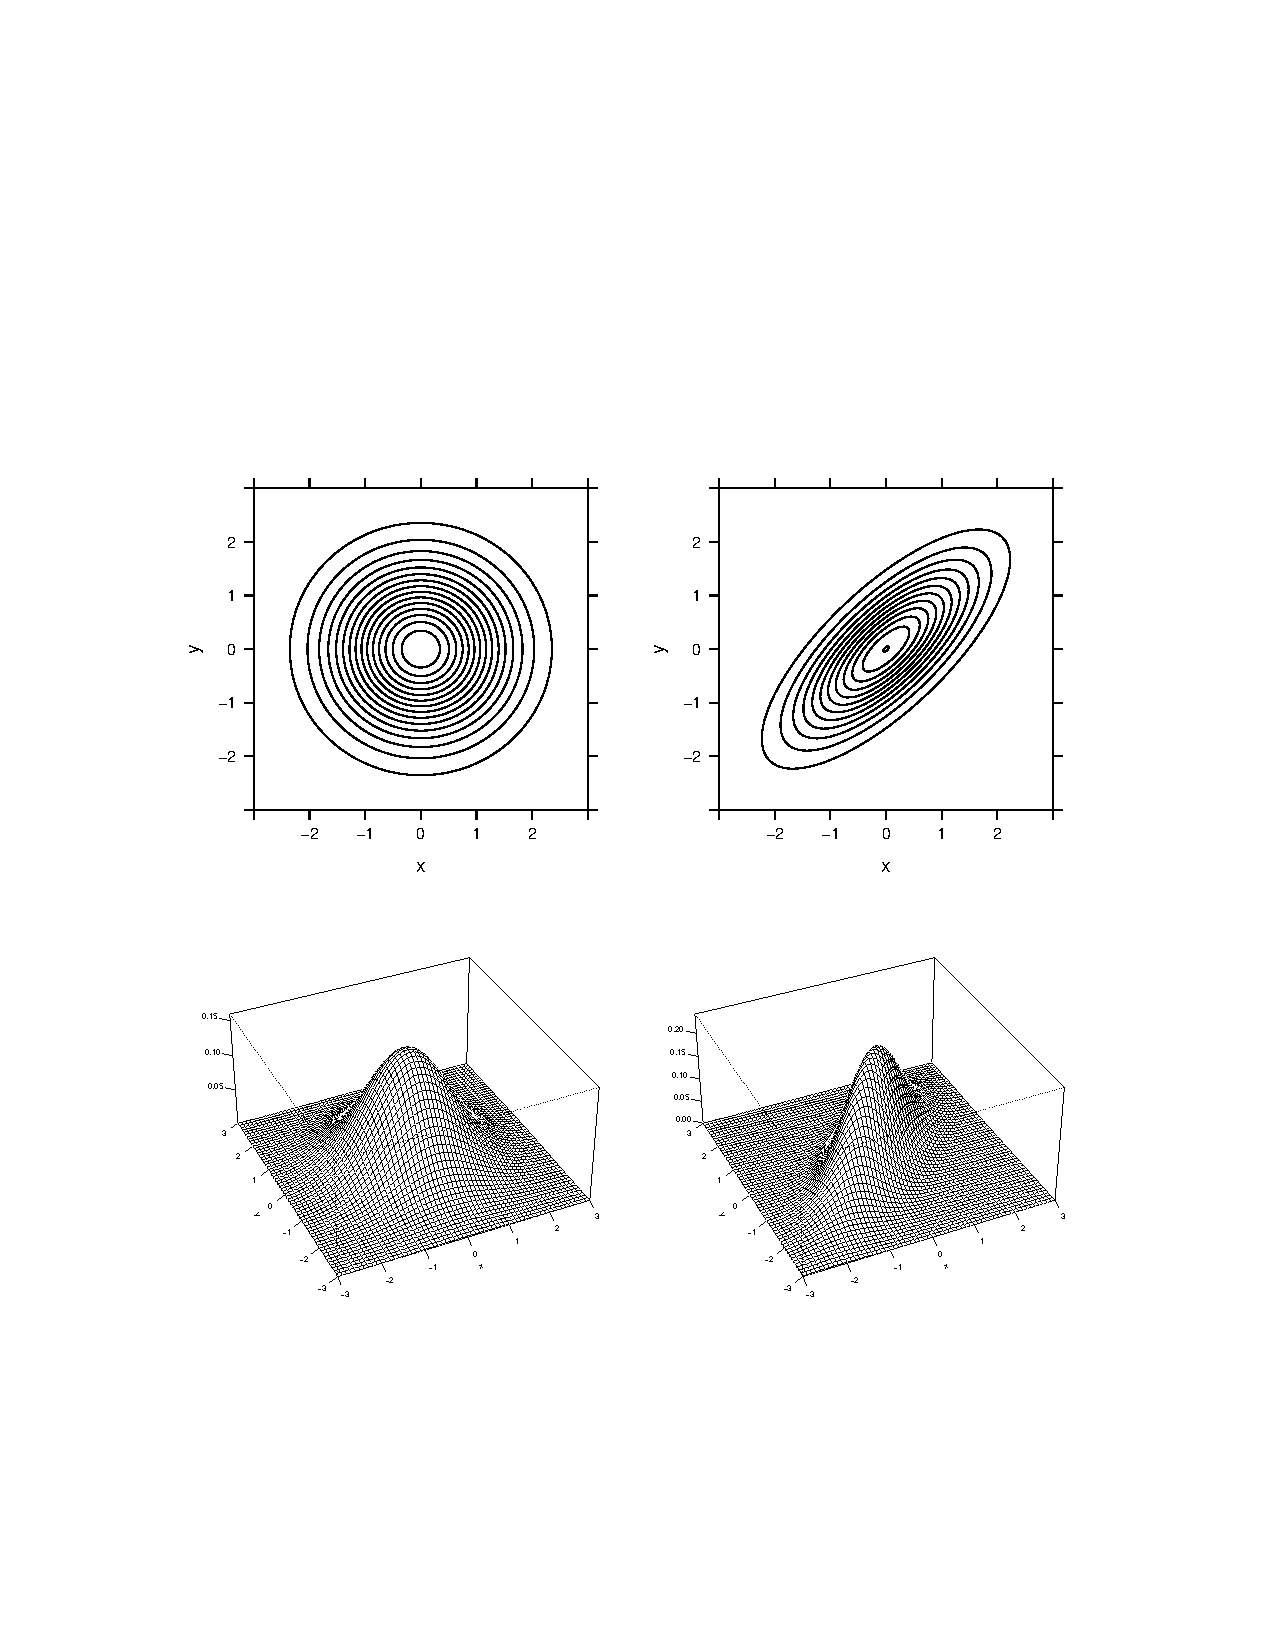
\includegraphics[width = \textwidth]{covariance.pdf}
\caption{(left) We have two uncorrelated distributions that are marginally identical. (right) We have two positively correlated distributions that are marginally identical. If we know that one of them is high relative to the mean, then we know that the the other one is likely to be high relative to the mean too. Plots courtesy of Jessy Hwang.}
\end{figure}

\newpage

\section*{Covariance and Correlation (cont'd)}
\begin{description}
\item [Covariance] is the two-random-variable equivalent of Variance, defined by the following:
	\[\cov(X, Y) = E[(X - E(X))(Y - E(Y))] = E(XY) - E(X)E(Y)\]
	Note that 
	\[\cov(X, X) = E(XX) - E(X)E(X) =  E(X^2) - [E(X)]^2 = \var(X)\]
\item [Correlation] is a rescaled variant of Covariance that is always between -1 and 1.
	\[\corr(X, Y) = \frac{\cov(X, Y)}{\sqrt{\var(X)\var(Y)}} = \frac{\cov(X, Y)}{\sigma_X\sigma_Y}\]
\item [Covariance and Indepedence] - If two random variables are independent, then they are uncorrelated. The inverse is not necessarily true. 
	\[X \independent Y \longrightarrow \cov(X, Y) = 0\]

%, except in the case of Multivariate Normal, where uncorrelated \emph{does} imply independence.
\item [Covariance and Variance] - Note that
	\begin{align*}
		\cov(X, X) &= \var(X) \\
		\var(X + Y) &= \var(X) + \var(Y) + 2\cov(X, Y) \\
		\var(X_1 + X_2 + \dots + X_n ) &= \sum_{i = 1}^{n}\var(X_i) + 2\sum_{i < j} \cov(X_i, X_j)
	\end{align*}
	In particular, if X and Y are independent then they have covariance 0 thus
	\[X \independent Y \Longrightarrow \var(X + Y) = \var(X) + \var(Y)\]
	In particular, If $X_1, X_2, \dots, X_n$ are i.i.d. and all of them have the same covariance relationship, then 
	\[\var(X_1 + X_2 + \dots + X_n ) = n\var(X_1) + 2{n \choose 2}\cov(X_1, X_2)\]
	
\item [Covariance and Linearity] - For random variables $W, X, Y, Z$ and constants $b, c$:
	\begin{align*}
		\cov(X + b, Y + c) &= \cov(X, Y) \\
		\cov(2X, 3Y) &= 6\cov(X, Y) \\
		\cov(W + X, Y + Z) &= \cov(W, Y) + \cov(W, Z) + \cov(X, Y) + \cov(X, Z)
	\end{align*}
\item [Covariance and Invariance] - Correlation, Covariance, and Variance are addition-invariant, which means that adding a constant to the term(s) does not change the value. Let $b$ and $c$ be constants.
	\begin{align*}
		\var(X + c) &= \var(X) \\
		\cov(X + b, Y + c) &= \cov(X, Y) \\
		\corr(X + b, Y + c) &= \corr(X, Y) 
	\end{align*}
	In addition to addition-invariance, Correlation is \emph{scale-invariant}, which means that multiplying the terms by any constant does not affect the value. Covariance and Variance are not scale-invariant.
	\[\corr(2X, 3Y) = \frac{\cov(2X, 3Y)}{\sqrt{\var(2X)\var(3Y)}} = \frac{6\cov(X, Y)}{\sqrt{36\var(X)\var(Y)}} = \frac{\cov(X, Y)}{\sqrt{\var(X)\var(Y)}} = \corr(X, Y)\]
\item[Intuitive Explanation of Covariance] - See \\
\url{https://www.quora.com/Probability/What-is-an-intuitive-explanation-of-covariance}
\end{description}

\end{notes}

\newpage

\section*{Practice Problems} 

\begin{comment}
%%%%%%%%%%%%%%%%%%%%%%%%%%%%%%%%%%%%%%%%%%%%%%%%%%%%%%%%%%%

\begin{exercise}{Probabilities Using Joint CDFs and PDFs}
Let $X$ and $Y$ be continuous random variables. What is the probability that $(X, Y)$ falls into the 2-D rectangle $[a_1, a_2] \times [b_1, b_2]$ in terms of a) the joint CDF of $X$ and $Y$, $F(x, y)$, and b) the joint PDF of $x$ and $Y$, $f(x, y)$?
\end{exercise}

\begin{solution}{4}
\vspace{-5mm}
\begin{enumerate}
\item $F(a_2, b_2) - F(a_1, b_2) - F(a_2, b_1) + F(a_1, b_1)$. Draw a picture to see this.
\item We can integrate the joint PDF over the region of interest to get the probability:
$$P\paren{(X, Y) \in [a_1, a_2] \times [b_1, b_2]} = \int_{b_1}^{b_2} \int_{a_1}^{a_2} f(x, y) \diff x \diff y$$
\end{enumerate}
\end{solution}

%%%%%%%%%%%%%%%%%%%%%%%%%%%%%%%%%%%%%%%%%%%%%%%%%%%%%%%%%%%

\begin{exercise}{Discrete max and min} 
Let $X$ and $Y$ be i.i.d. $\Pois(\lambda)$, $L = \min(X, Y)$, and $M = \max(X, Y)$. Find the joint PMF of $L$ and $M$. Are $L$ and $M$ independent?
\end{exercise} 

\begin{solution}{4} 
We want $P(L = l, M = m)$ for all pairs $(l, m)$. Let's consider the three cases.
\begin{enumerate}[label=\arabic*.]
\item $l > m$: $P(L = l, M = m) = 0$
\item $l < m$:
\begin{align*}
P(L = l, M = m) &= P(X = l, Y = m) + P(X = m, Y = l) \\
&= 2 P(X = l, Y = m) & \textrm{by symmetry} \\
&= 2 P(X = l) P(Y = m) & \textrm{by independence of $X$ and $Y$} \\
&= 2 \frac{e^{-\lambda} \lambda^l}{l!} \frac{e^{-\lambda} \lambda^m}{m!}
\end{align*}
\item $l = m$:
\begin{align*}
P(L = l, M = m) &= P(L = l, M = l) \\
&= P(X = l, Y = l) \\
&= \paren{\frac{e^{-\lambda} \lambda^l}{l!}}^2
\end{align*}
\end{enumerate}
This fully specifies the joint PMF of $L$ and $M$. No, $L$ and $M$ are not independent. Knowning the value of $L$ constrains the possible values of $M$ and vice versa.
\end{solution}

\end{comment}

%%%%%%%%%%%%%%%%%%%%%%%%%%%%%%%%%%%%%%%%%%%%%%%%%%%%%%%%%%%

\begin{exercise}{Housing Day}
Suppose Harvard College is conducting its housing lottery. For simplicity's sake, we'll say that there are 1200 Freshmen that will be randomly assigned to 12 houses. Let $X_1, X_2, \ldots, X_{12}$ count how many students are place in Dunster ($X_1$), all the way to Pfoho ($X_{12}$) (organized by best house to worst).
\begin{enumerate}
\item Are $X_1$ and $X_2$ independent?
\item What is the joint distribution of $X_1, X_2, \ldots, X_{12}$?
\item What is the marginal distribution of $X_1$, the number of students who are placed into Dunster House, and the joint distribution of $X_1$ and $1200 - X_1$?
\item What is the conditional distribution of $X_1$ given $X_{10} + X_{11} + X_{12} = 450$?
\end{enumerate}
\end{exercise}

\begin{solution}{3.5}
\vspace{-5mm}
\begin{enumerate}
\item No they are not. Since the number of Freshmen is constrained to 1200, knowing that a lot of people got into one house decreases the number of people that could be in the remaining houses.
\item By the story of the Multinomial distribution,
$$(X_1, X_2, \ldots, X_{12}) \sim \Mult_{12}\paren{1200, \paren{1/12, \dots, 1/12}}$$
\item In this case, we can group together bins that are not in Dunster House together. We have
$$X_1 \sim \Bin\paren{1200, 1/12}$$
$$(X_1, 1200 - X_1) \sim \Mult_2\paren{1200, (1/12, 11/12)}$$
\item
$$X_1 | X_{10} + X_{11} + X_{12} = 450 \sim \Bin\paren{750, 1/9}$$
\end{enumerate}
\end{solution}

\begin{comment}
%%%%%%%%%%%%%%%%%%%%%%%%%%%%%%%%%%%%%%%%%%%%%%%%%%%%%%%%%%%

\begin{exercise}{Mixture distribution}
Suppose that either of two instruments might be used for making a certain measurement. Instrument 1 yields a measurement whose PDF is $h_1(x) = 2x$ for $0 < x < 1$ and 0 otherwise. Instrument 2 yields a measurement whose PDF is $h_2(x) = 3x^2$ for $0 < x < 1$ and 0 otherwise. Suppose that one of the two instruments is chosen at random and a measurement $X$ is made with it.
\begin{enumerate}
\item Determine the marginal PDF of $X$.
\item If the value of the measurement is $X = \frac{1}{4}$, what is the probability that instrument 1 was used?
\end{enumerate}
\end{exercise}

\begin{solution}{3}
\vspace{-5mm}
\begin{enumerate}
\item Let $I_1$ be the indicator of choosing instrument 1.
\begin{align*}
f_X(x) &= f_X(x | I_1 = 1) P(I_1 = 1) + f_X(x | I_1 = 0) P(I_1 = 0) \\
&= \frac{1}{2} h_1(x) + \frac{1}{2} h_2(x) \\
&= x + \frac{3}{2} x^2, \: 0 < x < 1
\end{align*}
\item Using Bayes' rule,
\begin{align*}
P\paren{I_1 = 1 | X = \frac{1}{4}} &= \frac{f_{X|I_1 = 1}\paren{\frac{1}{4}}P(I_1 = 1)}{f_X\paren{\frac{1}{4}}} \\
&= \frac{h_1\paren{\frac{1}{4}}P(I_1 = 1)}{f_X\paren{1/4}} \\
&= \frac{2 \cdot \frac{1}{4} \cdot \frac{1}{2}}{\frac{1}{4} + \frac{3}{2} \cdot \paren{\frac{1}{4}}^2} \\
&= \frac{8}{11}
\end{align*}
\end{enumerate}
\end{solution}

%%%%%%%%%%%%%%%%%%%%%%%%%%%%%%%%%%%%%%%%%%%%%%%%%%%%%%%%%%%

\begin{exercise}{Working with a Joint PDF}
The joint density function of $X$ and $Y$ is $f(x,y) = x+y$, where $0 < x < 1 $ and $0 < y < 1$.
\begin{enumerate}
\item Are $X$ and $Y$ independent?
\item Find $P(X + Y > \frac{3}{2})$.
\item Find the conditional density $f(x|y)$.
\item Set up an integral to determine the expected value $E(XY)$.
\end{enumerate}
\end{exercise}

\begin{solution}{3}
\vspace{-5mm}
\begin{enumerate}
\item Note that if two continuous random variables are independent, their joint PDF must be the product of their marginal PDFs (think about why this is the case). So, we can check if $f_{X, Y}(x, y) = f_X(x) f_Y(y)$. \\
Here, we can find the marginal PDF of $X$. By symmetry, the marginal PDF of $Y$ takes the exact same form. The marginal PDF of $X$ is
$$f_X(x) = \int_0^1 f(x, y) \, dy = \int_0^1 \paren{x + y} \, dy = x + \frac{1}{2}$$
Note that $f_{X, Y}(x, y) = x + y \not= \paren{x + \frac{1}{2}} \paren{y + \frac{1}{2}} = f_X(x) f_Y(y)$, and so $X$ and $Y$ are not independent.
\item To calculate the probability, note that $X$ must be at least $\frac{1}{2}$ (because $Y$ can't be any greater than 1, so if $X$ is less than $\frac{1}{2}$, the sum cannot be greater than $\frac{3}{2}$). Consequently, we want to find the probability that $Y$ is greater than $\frac{3}{2} - X$ under the constraint that $Y < 1$. It follows then that
\begin{align*}
P\paren{X + Y > \frac{3}{2}} &= \int_{\frac{1}{2}}^{1} \int_{\frac{3}{2} - x}^1 \paren{x + y} \, dy \, dx \\
&= \frac{5}{24}
\end{align*}
\item Using the definition of conditional density, we know that
$$f_{X|Y}(x|y) = \frac{f_{X,Y}(x, y)}{f_Y(y)} = \frac{x + y}{y + \frac{1}{2}}$$
\item Using 2D LOTUS, this is really simple!
$$E(XY) = \int_0^1 \int_0^1 xy(x + y) \, dy \, dx$$
\end{enumerate}
\end{solution}

%%%%%%%%%%%%%%%%%%%%%%%%%%%%%%%%%%%%%%%%%%%%%%%%%%%%%%%%%%%

\begin{exercise}{A Tale of Two Exponentials}
Let $X$ and $Y$ be continuous positive random variables.
\begin{enumerate}
\item Express $P(X < Y)$ in terms of the joint PDF of $X, Y$. 
\item Let's say that independently, $X \sim \Expo(\lambda_1)$ and $Y \sim \Expo(\lambda_2)$. What is the joint PDF of X, Y?
\item What is $P(X < Y)$?	
\end{enumerate}
\end{exercise}

\begin{solution}{3}
\vspace{-5mm}
\begin{enumerate}
\item To find probabilities, we want to integrate over the joint density over the possible values of $x, y$ that we are interested in. In this case, $Y$ can be any number $y \in [0, 1)$ , and $X | Y = y$ can be any number $x \in [0, y)$. We do a double integral over these regions.
$$P(X < Y) = \int_0^\infty \int_0^y f(x, y) \, dx \, dy$$
\item Let $f(x)$ be the PDF of $X$ and $g(x)$ be the PDF of $Y$. Because they are independent, we have that the joint PDF is simply the product of the marginal PDFs.
$$f(x, y) = f_X(x)f_Y(y) = \lambda_1 e^{-\lambda_1 x} \lambda_2 e^{-\lambda_2 y}$$
\item Combining the results from the first two parts, we have
\begin{align*}
P(X < Y) &= \int_0^\infty \int_0^y f(x, y) \, dx \, dy \\
&= \int_0^\infty \int_0^y f_X(x) f_Y(y) \, dx \, dy \\
&= \int_0^\infty f_Y(y) \int_0^y f_X(x) \, dx \, dy \\
&= \int_0^\infty f_Y(y) \brack{\int_0^y f_X(x) \, dx} \, dy \\
&= \int_0^\infty f_Y(y) F_X(y) \, dy \\
\end{align*}
Now we can plug in values and solve, noting the facts that PDFs must integrate to 1.
\begin{align*}
&= \int_0^\infty \lambda_2 e^{-\lambda_2 y} \paren{1 - e^{-\lambda_1 y}} \, dy \\
&= \int_0^\infty \lambda_2 e^{-\lambda_2 y} \, dy - \int_0^\infty \lambda_2 e^{-\lambda_2 y} e^{-\lambda_1 y} \, dy \\
&= \int_0^\infty \lambda_2 e^{-\lambda_2 y} \, dy - \int_0^\infty \lambda_2 e^{-(\lambda_1 + \lambda_2) y} \, dy \\
&= 1 - \frac{\lambda_2}{\lambda_1 + \lambda_2} \int_0^\infty (\lambda_1 + \lambda_2) e^{-(\lambda_1 + \lambda_2) y} \, dy \\
&= 1 - \frac{\lambda_2}{\lambda_1 + \lambda_2} \\
&= \frac{\lambda_1}{\lambda_1 + \lambda_2} \\
\end{align*}
\end{enumerate}
\end{solution}

\end{comment}


%%%%%%%%%%%%%%%%%%%%%%%%%%%%%%%%%%%%%%%%%%%%%%%%%%%%%%%%%%%

\begin{exercise}{Subsets of MVNs}
Let ($X_1, X_2$) be BVN. Marginally, suppose that $X_1$ and $X_2$ are $\N(0,1)$, and $\corr(X_1, X_2) = \rho$. 
\begin{enumerate}
	\item Find the distribution of $X_1 - 3X_2$.
	\item Find $c$ such that $X_1-3X_2 \independent X_1 + cX_2$.
\end{enumerate}
\end{exercise}
\begin{solution}{4.5}
\begin{enumerate}
    \vspace{-5mm}
    \item Because $X_1 - 3 X_2$ is a linear combination of a BVN, we know that $X_1 - 3 X_2$ is Normally distributed. \\
    We also know that
    \begin{align*}
        E(X_1 - 3 X_2) & = 0 \\
        \var(X_1 - 3 X_2) &= \var(X_1) + \var(3 X_2) - 2 \cov(X_1, 3 X_2) = 10 - 6 \rho
    \end{align*}
    So it follows that $X_1 - 3 X_2 \sim \N(0, 10 - 6 \rho)$
    
    \item We know that $(X_1 - 3 X_2, X_1 + c X_2)$ is BVN, and within MVN, uncorrelated implies independent. So we just need to find $c$ in order for $\cov(X_1 - 3 X_2, X_1 + c X_2) = 0$.
    $$\cov(X_1 - 3 X_2, X_1 + c X_2) = \var(X_1) - 3 \cov(X_1, X_2) + c \cov(X_1, X_2) - 3c \var(X_2) = 1 - 3\rho + c \rho - 3c$$
    Setting the above equal to 0 and solving for $c$, we get that $c = \frac{1 - 3 \rho}{3 - \rho}$.
\end{enumerate}
\end{solution}

%%%%%%%%%%%%%%%%%%%%%%%%%%%%%%%%%%%%%%%%%%%%%%%%%%%%%%%%%%%

% \begin{exercise}{Uncorrelated sum and difference}
% Show that if X and Y are identically distributed, then $\cov\paren{X + Y, X - Y} = 0$.
% \end{exercise}
% \begin{solution}{4}
% We use the fact that Covariance is billinear to get: 
% \begin{align*}
% \cov\paren{X + Y, X - Y} &= \cov\paren{X, X} + \cov\paren{X, -Y} + \cov\paren{Y, X} + \cov\paren{Y, -Y} \\
% &= \var\paren{X} - \var\paren{Y} \\
% &= 0
% \end{align*}
% \end{solution}

%%%%%%%%%%%%%%%%%%%%%%%%%%%%%%%%%%%%%%%%%%%%%%%%%%%%%%%%%%%


% \begin{exercise}{Correlation lower bound}
% Let $X_1, \ldots, X_n$ be random variables such that $\var\paren{X_i} = 1$ for all $i$ and $\corr\paren{X_i, X_j} = \rho$ for all $i \not= j$. Show that $\rho \geq - \frac{1}{n - 1}$. \\
% \textit{Hint:} $\var\paren{X_1 + \ldots + X_n} \geq 0$
% \end{exercise}

% \begin{solution}{4.5}
% First we note that
% \begin{align*}
% \corr\paren{X_i, X_j} &= \frac{\cov\paren{X_i, X_j}}{\sqrt{\var\paren{X_i} \var\paren{X_j}}} \\
% \cov\paren{X_i, X_j} &= \rho
% \end{align*}
% Hence,
% \begin{align*}
% \var\paren{X_1 + \ldots + X_n} &= \sum_{i=1}^n \var\paren{X_i} + 2 \sum_{i < j} \cov\paren{X_i, X_j} \\
% &= \sum_{i=1}^n 1 + 2 \sum_{i < j} \rho \\
% &= n + 2 \binom{n}{2} \rho \\
% &= n + n \paren{n - 1} \rho \\
% n + n \paren{n - 1} \rho &\geq 0 \\
% \rho &\geq - \frac{1}{n - 1}
% \end{align*}
% as desired.
% \end{solution}

%%%%%%%%%%%%%%%%%%%%%%%%%%%%%%%%%%%%%%%%%%%%%%%%%%%%%%%%%%%

\begin{exercise}{Jellybeans}
I have a jar of 30 jellybeans: 10 red, 8 green, 12 blue. I draw a sample
of 12 jellybeans without replacement. Let $X$ be the number of red jellybeans in the sample, $Y$ the number of green jellybeans. Find $\cov(X, Y)$.
\end{exercise}

\begin{solution}{4}
Let $X = I_1 + \ldots + I_{12}$, and $Y = J_1 + \ldots + J_{12}$, where
\begin{align*}
I_i &= \begin{cases}
1 & \textrm{if $i$th jellybean in sample is red} \\
0 & \textrm{otherwise}
\end{cases} \\
J_i &= \begin{cases}
1 & \textrm{if $i$th jellybean in sample is green} \\
0 & \textrm{otherwise}
\end{cases}
\end{align*}
\begin{align*}
\cov\paren{I_1, J_1} &= E\paren{I_1 J_1} - E\paren{I_1} E\paren{J_1} \\
&= 0 - \paren{\frac{10}{30}}\paren{\frac{8}{30}} \\
\cov\paren{I_1, J_2} &= E\paren{I_1 J_2} - E\paren{I_1} E\paren{J_2} \\
&= \paren{\frac{10}{30}}\paren{\frac{8}{29}} - \paren{\frac{10}{30}}\paren{\frac{8}{30}} \\
\cov\paren{X, Y} &= \sum_{i=1}^{12} \cov\paren{I_i, J_i} + 2 \sum_{i < j} \cov\paren{I_i, J_j} \\
&= \sum_{i=1}^{12} \cov\paren{I_1, J_1} + 2 \binom{12}{2} \cov\paren{I_1, J_2} \\
&= 12 \cdot \cov\paren{I_1, J_1} + 12 \cdot 11 \cdot \cov\paren{I_1, J_2} \\
&= - \frac{96}{145}
\end{align*}
It's good to do a little sanity check at the end: it makes sense that the covariance is negative. If the sample contains a lot of red jellybeans, the sample probably has fewer green jellybeans. \\
Another way to solve this is to create an indicator for each red jellybean and each green jellybean in the jar, where the indicator equals 1 if the jellybean is in the sample and 0 otherwise.
\end{solution}

%%%%%%%%%%%%%%%%%%%%%%%%%%%%%%%%%%%%%%%%%%%%%%%%%%%%%%%%%%%

% \begin{exercise}{Correlation and Independence for Normals}
% Suppose $X$ and $Y$ are marginally Normal and are uncorrelated. Is it always true that $X+Y$ is a normal random variable? What if $X$ and $Y$ are also independent?
% \end{exercise}
% \begin{solution}{3.5}
% It is not necessarily true that X + Y is Normally distributed because $(X, Y)$ is not MVN (make sure you understand this statement)! As an example, suppose that $X \sim \N(0, 1)$ and $Y = SX$ where $S$ is a random sign (takes on a value of -1 or +1 which 0.5 probability each). $Y$ in this case is uncorrelated with $X$ (showing this is an exercise for the reader!) but $X + Y$ has a positive probability of equaling 0, so $X + Y$ definitely cannot be Normally distributed.
% \end{solution}

\begin{exercise}{Stat Courses}
Let $X$ be the number of statistics majors in a certain college in the class of 2030, viewed as an r.v. Each statistics major chooses between two tracks: a general track in statistical principles, and a track in quant finance. Suppose that each statistics major chooses randomly which of these two tracks to follow, independently, with probability $p$ of choosing the general track. Let $Y$ be the number of statistics majors who choose the general track, and $Z$ be the number of statistics majors who choose the quantitative finance track. 

\begin{enumerate}
    \item Suppose that $X \sim \text{Pois}(\lambda)$. Find the correlation between
    $X$ and $Y$.
    \item Let $n$ be the size of the Class of 2030, where $n$ is a known constant. For 
    this part and the next, instead of assuming that $X$ is Poisson, assume that each 
    of the $n$ students chooses to be a statistics major with probability $r$, 
    independently. Find the joint distributions of $Y$, $Z$, and the number of 
    non-statistics majors, and their marginal distributions. 
    \item Continuing as in the previous part, find the correlation between
     $X$ and $Y$. 
\end{enumerate}
\end{exercise}

\begin{solution}{4}

\begin{enumerate}
    \item By the chicken-egg story, we know that $Y$ and $Z$ are independent Poisson
    random variables, with rate parameters $\lambda p $ and $\lambda q$, respectively. 
    We must first find the covariance between $X$ and $Y$.
        $$Cov(X,Y) = Cov(Y+Z, Y) = Var(Y) + Cov(Y,Z) = \lambda p$$
    We now plug this into the equation for correlation:
        $$Corr(X,Y)  =\frac{Cov(X,Y)}{\sqrt{Var(X)Var(Y)}} = \frac{\lambda p}{
        \sqrt{\lambda \lambda p}} = \sqrt{p} $$
    \item Under this new model, we have that $X\sim \text{Bin}(n,r)$. By the 
    multiplication rule, we have that the probability of a student becoming
    a general Statistician is $rp$, a Goldman-Sachs Statistician is $rq$, and a 
    non-Statstician (lame) is $1-r$. Therefore, we can apply the story of the
    Multinomial here:
        $$(Y, Z, n-X) \sim Mult_3(n, (rp, rq, 1-r)) $$
    \item We use the fact that covariance of the marginal distributions in a 
    multinomial is given by $-np_i p_j$.
        $$Cov(X,Y) = Cov(Y+Z, Y) = Var(Y) + Cov(Z,Y) = nrp(1-rp) - n(rp)(rq) 
        =npr(1-r)$$
\end{enumerate}
\end{solution}

%%%%%%%%%%%%%%%%%%%%%%%%%%%%%%%%%%%%%%%%%%%%%%%%%%%%%%%%%%%



\end{document}
